\documentclass[tikz]{standalone}
% \usepackage{tikz} % already loaded by the documentclass


\begin{document}
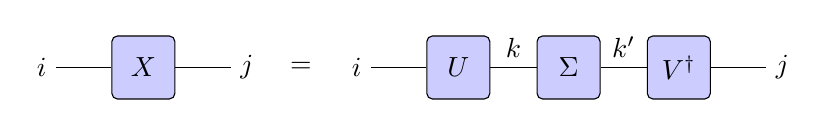
\begin{tikzpicture}[
    tensor/.style={draw,fill=blue!20,rounded corners=2pt,minimum size=8mm},
  ]
  \node[tensor] (X) at (0,0) {$X$};
  \draw (X.west) -- ++(-0.7,0) node[left]{$i$};
  \draw (X.east) -- ++(0.7,0) node[right]{$j$};
  \node at (2,0) {$=$};
  \node[tensor] (U) at (4,0) {$U$};
  \node[tensor] (S) at (5.4,0) {$\Sigma$};
  \node[tensor] (V) at (6.8,0) {$V^\dagger$};
  \draw (U.west) -- ++(-0.7,0) node[left]{$i$};
  \draw (U.east) -- (S.west) node[midway,above]{$k$};
  \draw (S.east) -- (V.west) node[midway,above]{$k'$};
  \draw (V.east) -- ++(0.7,0) node[right]{$j$};
\end{tikzpicture}
\end{document}
      